\chapter{Requirements}
\label{chapter-Requirements}

This chapter is divided into two sections.
Section \ref{section-RequirementseZPublish3} presents the workflow mechanism
that is part of eZ~Publish~3, the current version of the Enterprise Content
Management System by eZ~Systems~AS. Section \ref{section-RequirementseZPublishTelemark}
discusses the requirements that the workflow engine for eZ~Publish~Telemark,
the next version of eZ~Publish, needs to fulfill.

\section{eZ Publish 3}
\label{section-RequirementseZPublish3}

eZ~Publish~3 comes with an integrated workflow mechanism that makes it
possible to perform different tasks with or without user interaction.

\begin{figure}[hbt]
\begin{center}
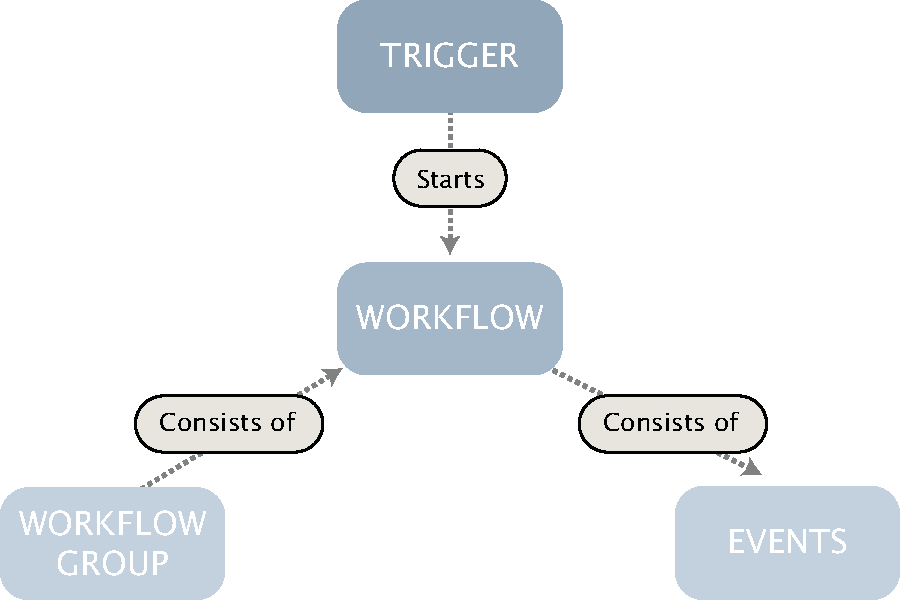
\includegraphics[width=10cm]{figures/WorkflowEZPublish3}\\[5mm]
\end{center}
\caption{The workflow system in eZ Publish 3}
\label{figure-WorkflowEZPublish3}
\end{figure}

Figure~\ref{figure-WorkflowEZPublish3} shows the components that comprise this
mechanism.

An \emph{event} performs a specific task. eZ~Publish~3 ships with a library
of events and custom events can be implemented in PHP.

A \emph{workflow} defines an ordered sequence in which workflow events are
executed and is initiated by a \emph{trigger} that is associated with a
function of a module (see Section~\ref{section-eZPublish}). It will start the
specified workflow either before or after that function has finished
executing.

\begin{figure}[hbt]
\begin{center}
\begin{tikzpicture}
  \node at (-6, 4) [activity] (ChooseClass) {Choose class};
  \node at ( 0, 4) [activity] (ChooseLanguage) {Choose language};
  \node at ( 0, 2) [activity] (CreateObject) {Create object};
  \node at (-6, 0) [activity] (StoreInput) {Store input};
  \node at ( 0, 0) [activity] (DisplayEditor) {Display editor};
  \node at ( 6, 1) [activity] (Browse) {Browse for existing object};
  \node at ( 6,-1) [activity] (Add) {Add selected object};
  \node at ( 0,-2) [activity] (CreateDraft) {Create new draft};
  \node [rectangle,draw=green!50,fill=green!20,thick] at (-6,-2) (Publish) {Publish in tree};
  \node at (-3,-4) [activity] (DisplayParent) {Display parent location};
  \draw [->] (ChooseClass) to (ChooseLanguage);
  \draw [->] (ChooseClass) to (CreateObject);
  \draw [->] (ChooseLanguage) to (CreateObject);
  \draw [->] (CreateObject) to (DisplayEditor);
  \draw [->] (DisplayEditor) to (StoreInput);
  \draw [->] (StoreInput) to (DisplayEditor);
  \draw [->] (Browse) to (DisplayEditor);
  \draw [->] (DisplayEditor) to (Browse);
  \draw [->] (Browse) to (Add);
  \draw [->] (Add) to (DisplayEditor);
  \draw [->] (CreateDraft) to (DisplayEditor);
  \draw [->] (DisplayEditor) to (Publish);
  \draw [->] (Publish) to (DisplayParent);
  \draw [->] (DisplayParent) to (CreateDraft);
\end{tikzpicture}
\end{center}
\caption{Workflow for publishing a content object in eZ Publish 3}
\label{figure-PublishObjectWorkflow}
\end{figure}

Figure \ref{figure-PublishObjectWorkflow} shows the built-in workflow for
publishing acontent object in eZ~Publish~3. This workflow can only be
customized at the \emph{Publish in tree} activity. This activity serves as the
trigger for a custom workflow that can be executed either before or after the
activity was executed.

\section{eZ Publish Telemark}
\label{section-RequirementseZPublishTelemark}

Both the architecture of the current eZ~Publish version as well as its
workflow feature have shortcomings that are to be overcome:

\begin{itemize}
\item Only some operations are workflows. This inconsistency has a negative
      effect on the maintainability of the software as a whole.
\item It is not easy to configure (hook in) the (internal) workflows. This
      makes extending the software hard.
\item Support for checking the state of executing workflows and control
      over them is limited.
\item Support for conditions is limited.
\end{itemize}

Eventually, the workflow component should become an important part of the
overall solution. However, it must not be tightly integrated or too much
dependent on other parts of the system (and vice versa). This means that
the workflow component must be flexible and provide good interfaces which
allow it to co-exist and plug into the software.

Georgakopoulos et. al. list general requirements for workflow management
systems:

\begin{quote}
\emph{To effectively support [workflow management], organizations must evolve
their existing computing environments to a new distributed environment that:
is \emph{component-oriented}, i.e. supports integration and interoperability
among loosely-coupled components [...], supports \emph{workflow applications}
corresponding to business or information process implementations [...],
ensures the correctness and reliability of applications in the presence of
concurrency and failures, and supports the evolution, replacement, and
addition of workflow applications and component systems as processes are
reengineered} \cite{DG95}.
\end{quote}

Following are the requirements set up by eZ~Systems~AS. We start with the
requirements that are relevant to the underlying workflow model of the
workflow component that is to be implemented:

\begin{itemize}
\item The workflow component should provide good support for expressing
      control flow using the workflow patterns (see
      Chapter~\ref{chapter-WorkflowModel}).
\item Any non-trivial operation in eZ~Publish, for instance the publishing,
      removal, and modification of content objects, should be a expressable
      through workflows.
\item Workflows should be composable through a concept of sub-workflows.
\end{itemize}

Now we come to the requirements that relate to the actual software
implementation:

\begin{itemize}
\item The workflow component has to be implemented using version 5 of the
      PHP programming language.
\item It should be possible to integrate workflows with the background
      processes of eZ~Publish (run workflow as background process, interact
      with a background process).
\item The workflow component should be customizable and extendable.
\item The data storage (for workflow schemas and the persistence of
      workflow instances) should be abstracted, relational databases must
      be supported as one backend.
\item Versioning of workflow schemas should be supported.
\item It should be possible to get information on the workflow instances
      that are currently executing.
\item It should be possible to manually control the workflow instances
      that are currently executing.
\item Simulation of workflow execution for debugging and testing purposes
      should be possible.
\end{itemize}

\subsection{Use Cases}

Here are two use cases that should be supported by the workflow engine
component that is to be implemented for eZ~publish Telemark as part of this
thesis. They are currently implemented using custom extensions for
eZ~publish~3.

\subsubsection{Multiple Approval, ISO Certification}

This scenario is from a current customer of the eZ~Publish ECMS providing
quality assurance for dairy products. The customer has information about
the dairy products stored in eZ~Publish. When they update any content
there is a strict ISO-governed process to follow. This process basically
consists of a \emph{five-level approval}:

\begin{itemize}
\item Bertrand produces an article.
\item Approver Level 1: B�rd decides who the next four approvers are.\\
      He can also edit the article and send it back to its creator.
\item Approver Level 2: Melissa reviews the article for political
      correctness.\\
      She can edit the article and send it back one level.
\item Approver Level 3: Vidar reviews the article for sales arguments.\\
      He can edit the article and and send it back one level.
\item Approver Level 4: Jennifer does grammar checks on the article.\\
      She can edit the article and and send it back one level.
\item Publisher: Markus approves the final article and chooses the time
      and location for publication.
\end{itemize}

\begin{figure}[hbt]
\begin{center}
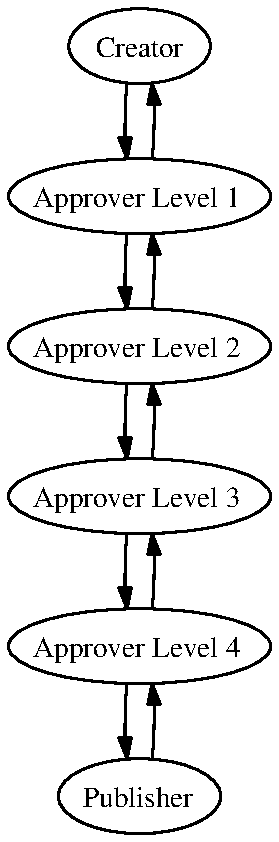
\includegraphics[height=10cm]{figures/MultipleApproval}\\[5mm]
\end{center}
\caption{The \emph{Multiple Approval} workflow}
\label{figure-MultipleApproval}
\end{figure}

It is possible to see all on-going processes for an administrator. He or
she can see each article as well as its state and which person currently
handles it.

\subsubsection{Employment Process}

This scenario is from the intranet of a current customer of the eZ~Publish
ECMS and is used when a new employee is hired.

\begin{itemize}
\item One person creates an Employee object (including name, address,
      email, etc.).
\item An e-mail with a link for final approval of the employment is
      sent to the CEO.
\item Once the CEO has approved the new employment three parallel
      activities are started:
      \begin{itemize}
      \item An e-mail to the system administrator is sent with the
            request to create e-mail and other accounts.\\
            The e-mail contains a link for the system administrator to
            click when he is done.
      \item An automatic process is started to set up accounts on
            different systems.
      \item An e-mail to the administration is sent with the request
            to buy new hardware for the new employee.
      \end{itemize}
\item Once these three activities have been completed, the workflow
      continues.
\item The Employee object is published.
\item An e-mail with detailed information is sent to the new employee.
\end{itemize}

\begin{figure}[hbt]
\begin{center}
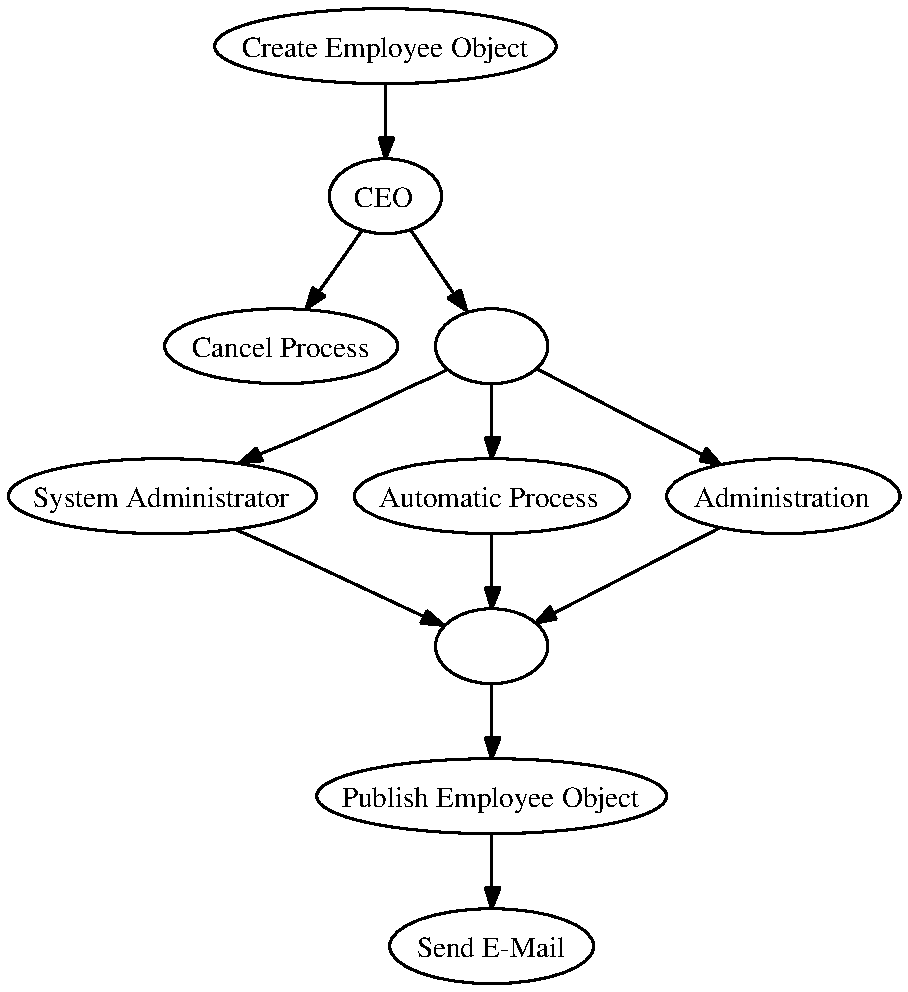
\includegraphics[height=10cm]{figures/EmploymentProcess}\\[5mm]
\end{center}
\caption{The \emph{Employment Process} workflow}
\label{figure-EmploymentProcess}
\end{figure}

The on-going status for all employment processes at any time is available
to anyone with the appropriate permissions.

\section{Summary}

This chapter discussed the requirements for the software that has been
developed as part of this thesis. This software will replace the workflow
engine of eZ~Publish~3 which has severe limitations with regard to the
underlying workflow model (only one directly supported workflow pattern)
and the software implementation (not easily extendable).
